\documentclass[12pt, a4paper]{ntut-report}
\usepackage[dvips,xetex]{graphicx}
\usepackage{ifpdf,mla}
\usepackage{geometry}
\usepackage{lipsum}
\usepackage{xeCJK}
\usepackage{wallpaper}
\usepackage{pdfpages}
\usepackage{indentfirst}
\usepackage{setspace}
\usepackage{hyperref}
\usepackage{zhnumber}
\usepackage{titlesec}
\usepackage{amsmath}

% --- 路線一：使用現代版 biblatex 處理 APA 格式 ---
% 特別加上 backend=biber 確保編譯器抓取正確
\usepackage[style=apa, backend=biber]{biblatex}
\usepackage{tabularx}
\usepackage{csquotes}
\usepackage{subcaption}

\MakeAutoQuote{“}{”}
\MakeOuterQuote{"}

\captionsetup{justification=centering,singlelinecheck=false,font={normalsize,stretch=2}}
\captionsetup[sub]{justification=centering,singlelinecheck=false,font={normalsize,stretch=2}}

\renewcommand{\baselinestretch}{1.5}
\xeCJKsetup{AutoFakeBold=true, AutoFakeSlant=true}
\setCJKmainfont{DFKai-SB.ttf} % 中文字體 (標楷體)
\setmainfont{Times New Roman} % 英文字體

% 將邊界統一設定為政大要求的 2.54cm
\geometry{a4paper,top=2.54cm,bottom=2.54cm,left=2.54cm,right=2.54cm} 
\pagestyle{plain} % 頁碼

% 讀取你的文獻資料庫 (確保 reference.bib 放在與 main.tex 同一層目錄)
\addbibresource{reference.bib}

\input{ntut-labels.tex}

\begin{document}

% 1. 封面 (已拿掉北科大原本多餘的空白頁與雙封面)
\begin{titlepage}
\begin{center}

\vspace*{\fill} 

% 1. 校系名稱 (18號字，標楷體)
{\fontsize{18pt}{27pt}\selectfont 國立政治大學\deptCname\par}

\vspace{\fill} 

% 2. 學位別 (20號字，標楷體)
{\fontsize{20pt}{30pt}\selectfont \degreeCname 學位論文\par}

\vspace{\fill} 

% 3. 中文題目 (20號字，標楷體)
{\fontsize{20pt}{30pt}\selectfont \cTitle\par}

\vspace{0.8cm} 

% 4. 英文題目 (16號字，Times New Roman)
{\fontsize{16pt}{24pt}\usefont{T1}{ptm}{m}{n}\selectfont \eTitle\par}

\vspace{\fill} 

% 5. 指導教授與研究生姓名 (18號字，標楷體)
{\fontsize{18pt}{27pt}\selectfont 指導教授：\advisorCname \ 博士\par}
\vspace{0.3cm}
{\fontsize{18pt}{27pt}\selectfont 研究生：\myCname \ 撰\par}

\vspace{\fill} 

% 6. 口試通過年月 (18號字，標楷體)
% 這裡在「年」跟「\cMonth」之間加上了 \ 來強制空一格
{\fontsize{18pt}{27pt}\selectfont 中華民國\ \cYear{} \ 年\ \cMonth{}\ 月\par}

\vspace*{\fill} 

\end{center}
\end{titlepage}

% 2. 授權書 (政大規定要在審定書前面，請把從系統印出的 PDF 放入 static-page 資料夾並解開下方註解)
% \includepdf[pages=-]{static-page/authorization.pdf}

% 3. 學位論文口試委員會審定書
% 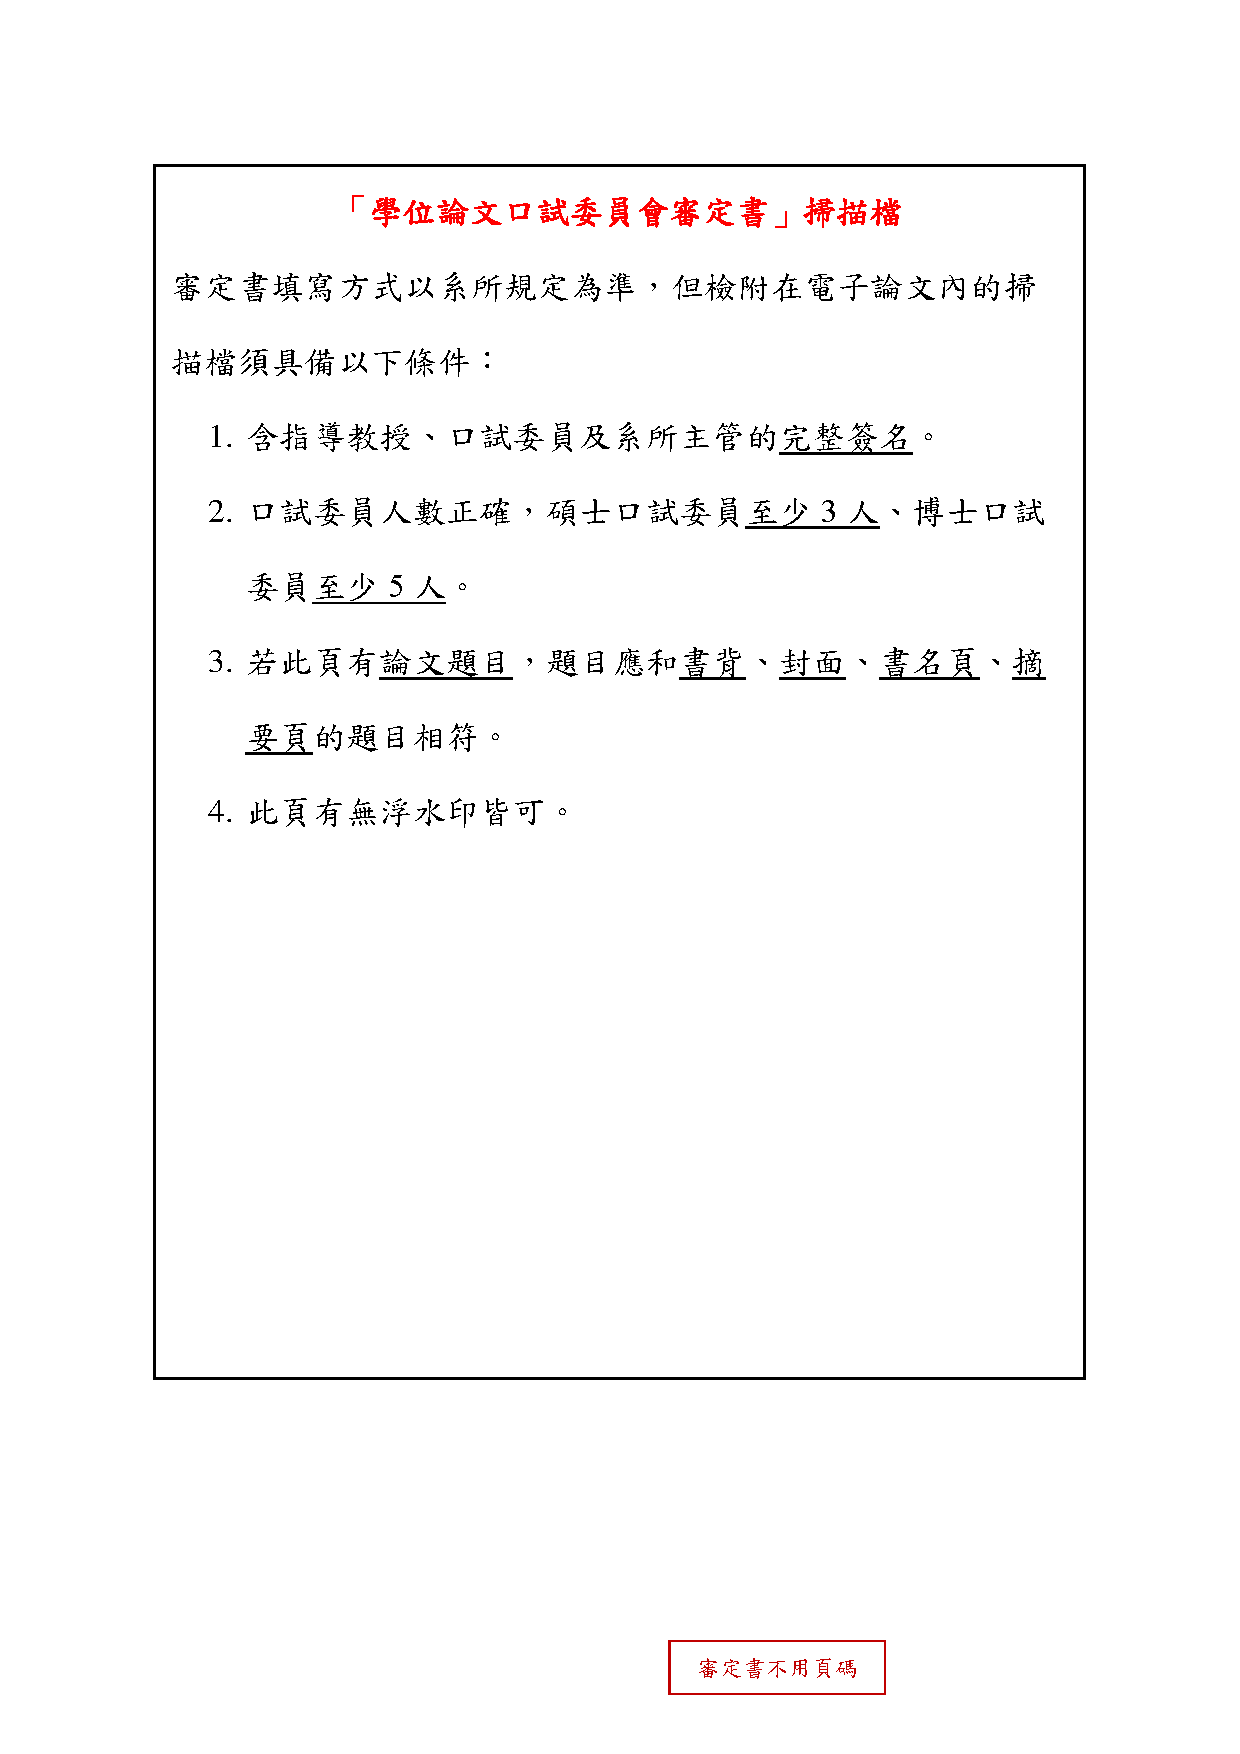
\includepdf[pages=-]{static-page/signpage.pdf}

\pagenumbering{roman}

% 4. 謝辭 (政大規定謝辭必須在摘要之前)
\include{page/thanks.tex}

% 5. 摘要頁（中文）
\include{page/abstract.tex}

% 6. 摘要頁（英文）
\include{page/abstract-en.tex}

% 7. 目次、表次與圖次
\include{page/table-of-content.tex}
 
\pagenumbering{arabic}

% 正文章節
\include{chapter/chapter1-introduction.tex}
\include{chapter/chapter2-related-work.tex}
% 新增你自己的章節... Add chapters here

% 8. 參考文獻 (使用 include 呼叫設定好的 reference.tex)
% \addcontentsline{toc}{chapter}{參考文獻}
% \renewcommand{\bibname}{參考文獻}

\clearpage
\phantomsection

% 強制印出 reference.bib 裡面的所有文獻（即使正文還沒用 \cite 引用也會印出來）
% 等到未來正文寫完且都有確實引用後，可以把 \nocite{*} 這行註解掉
\nocite{*} 

% 印出 APA 格式的參考文獻，並自動將「參考文獻」加入目錄中
\printbibliography[title={參考文獻}, heading=bibintoc]

\end{document}